\documentclass{article}
\usepackage[utf8]{inputenc}
\usepackage{amsmath}
\usepackage{amssymb}
\usepackage{graphicx}


\begin{document}
\section*{Matrix-Vector Product in CRS format}
We are given the following compressed row storage format.
\begin{figure}[!hbt]
    \centering
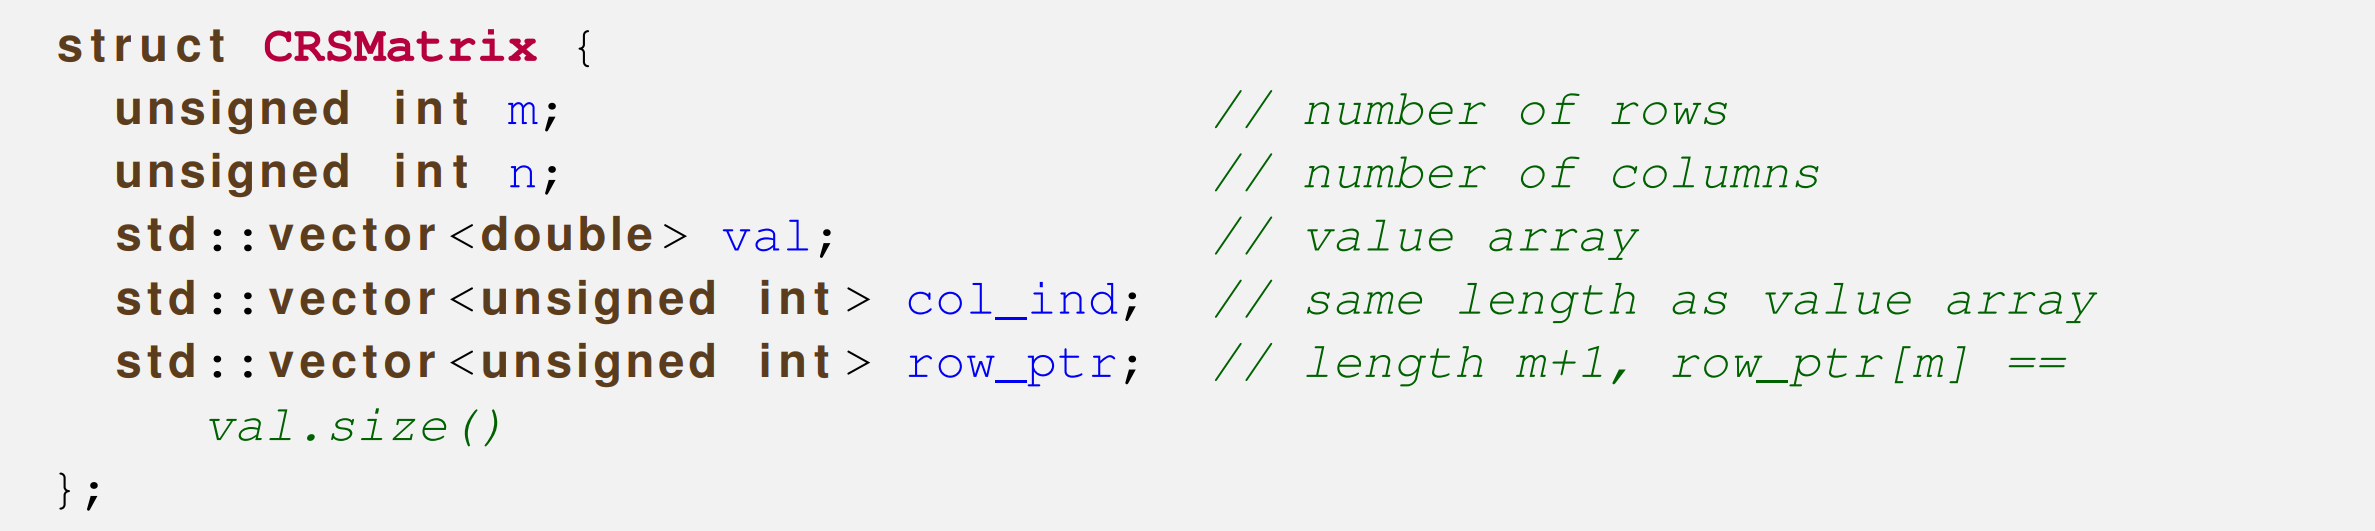
\includegraphics[width=1.0\linewidth]{CRSFormatExercise.png}
\end{figure}
The format is then defined by the following relationship (here $0$-indexed)
\begin{equation*}
    \text{val}\left[k\right] = a_{ij} \Longleftrightarrow 
    \begin{cases}
        \text{col\_ind}\left[k\right]& = j \\
        \text{row\_ptr}\left[i\right] &\leq k < \text{row\_ptr}\left[i+1\right]
    \end{cases} \quad 0 \leq k \leq \text{val}.\text{size}\left(\right)
\end{equation*}
for $i \in \left\{0, \dots, m-1\right\}$, $j \in \left\{0, \dots, n-1\right\}$
\subsection*{2-20.a}
The function \verb|crsmv| is supposed to return the product of a matrix in CRS format passed through \verb|M| and of a vector given as argument \verb|x|. The following code skeleton is given and we are supposed to supplement the missing parts.

\begin{figure}[!hbt]
    \centering
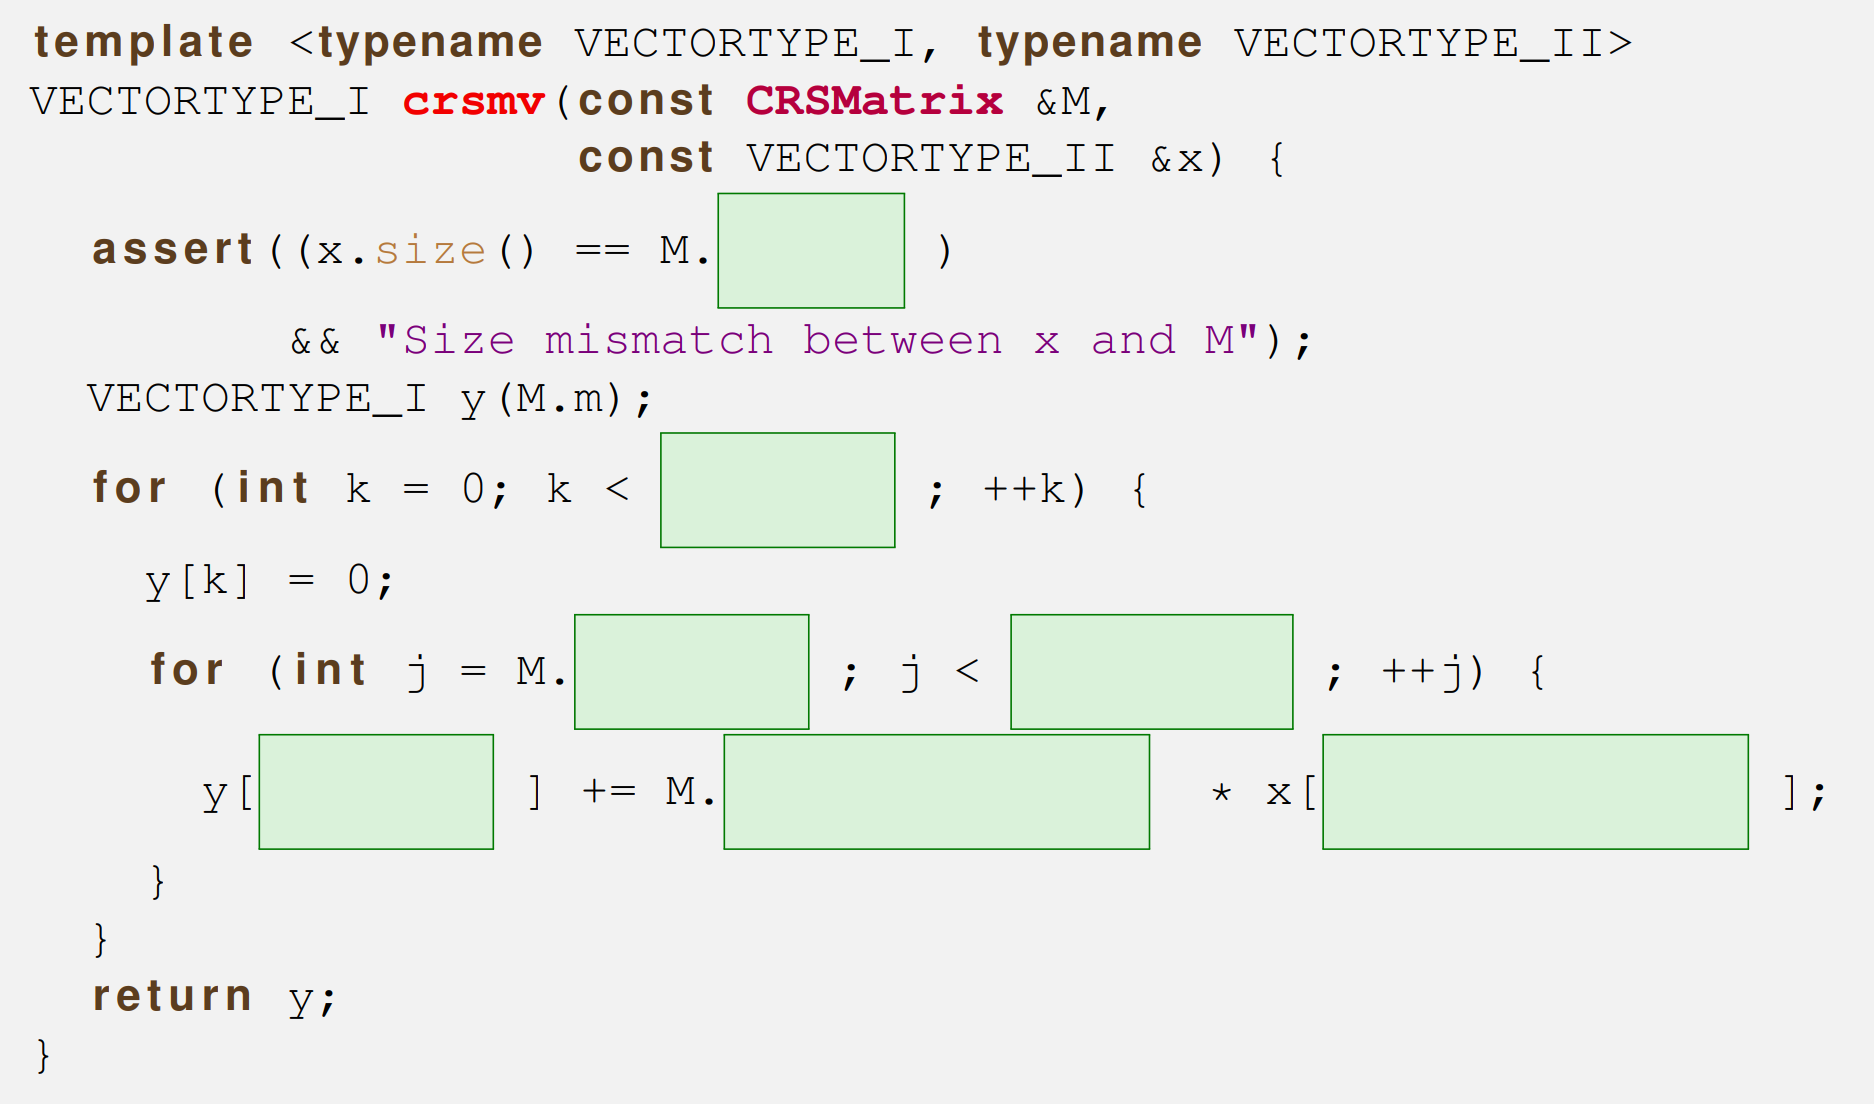
\includegraphics[width=1.0\linewidth]{CRSMatrix.png}
\end{figure}
\noindent The first box is supposed to contain \verb|M.n| as we need \verb|x| to have the same amount of entries as \verb|M| has columns for the matrix-vector product to work. The second box contains a restriction on how big \verb|k| should get, seeing as this is probably used for the  \verb|row_ptr| array we fill the box with \verb|k < M.m|. The third box then gives us the range in \verb|col_ptr| which is given by \verb|j = M.row_ptr[k]| to \verb|j < M.row_ptr[k+1]|. We then have that the element sits at the row $k$ and thus the fifth box is filled with \verb|y[k]|, where we access the element in the \verb|val_ptr| array according to the $j$-th entry of the \verb|col_ptr| array, hence we have as the sixth entry \verb|M.val.at(j)| (\verb|col_index| and \verb|val| have same length and map directly to each other) and multiply this with the corresponding row of \verb|x|, hence the seventh entry is \verb|x[M.col_ind[j]]| (which gives us the columns of the corresponding element). 
\begin{figure}[!hbt]
    \centering
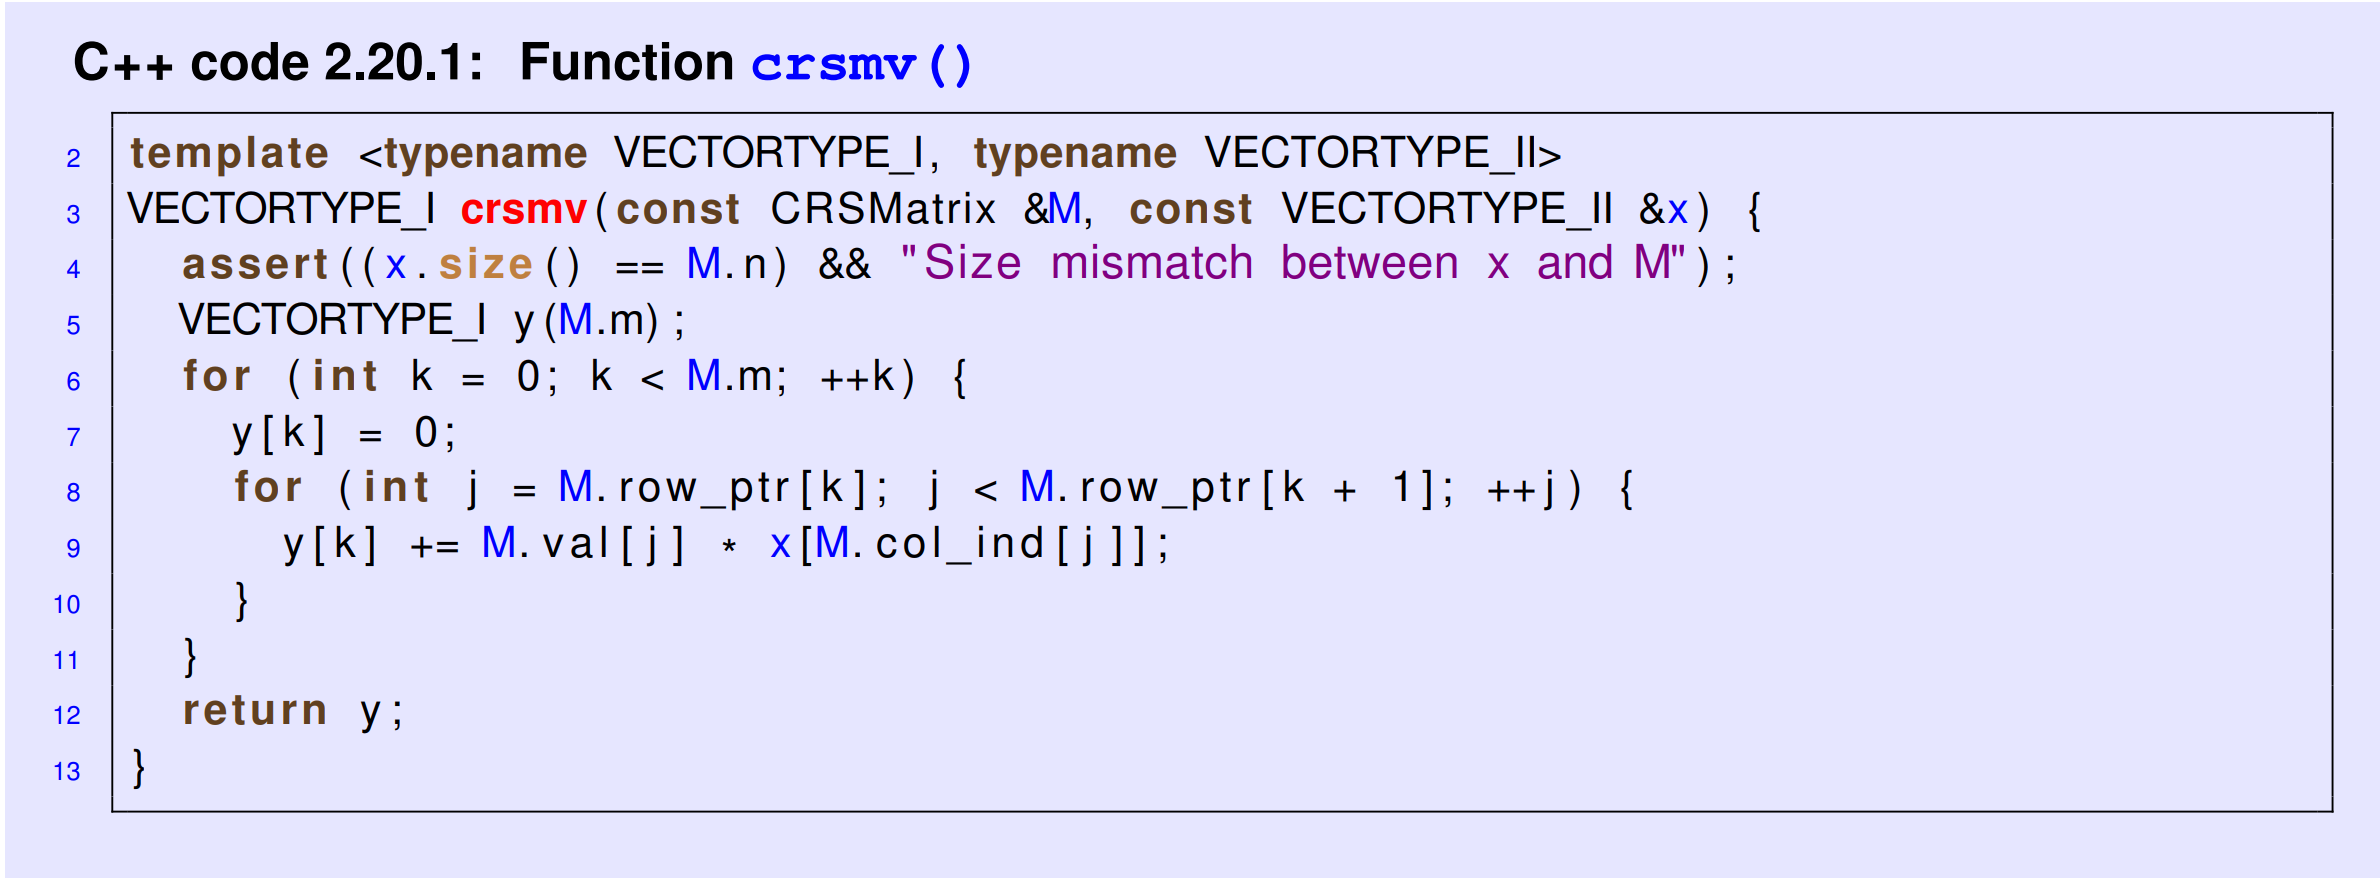
\includegraphics[width=1.0\linewidth]{CRSMatVectSol.png}
\end{figure}
\end{document}
